\documentclass[10pt]{beamer}

\usetheme{metropolis}
\usepackage{appendixnumberbeamer}
\usepackage{booktabs}
\usepackage[scale=2]{ccicons}
\usepackage{pgfplots}
\usepackage{color}
\usepgfplotslibrary{dateplot}
\usepackage{xspace}
\newcommand{\themename}{\textbf{\textsc{metropolis}}\xspace}

\usepackage{stmaryrd}
\usepackage{amsmath}
\usepackage{verbatim}
\usepackage{tikz}
\usepackage{siunitx}
\usepackage{color}
\usepackage[normalem]{ulem}
\usetikzlibrary{calc,decorations.pathmorphing,patterns}
\usepackage{amssymb}
\usepackage{amsfonts}
\usepackage{amscd}
\usepackage{amsthm}
\usepackage{mathrsfs}
\usepackage{enumerate}
\usepackage{mathtools}
\usepackage{booktabs}
\usepackage{array}
\usepackage{nth}
\usepackage{lipsum}


%%%%%%%%%%%%%%%%%%%%%%%%%%%%%list %%%%%%%%%%%%%%%%%
\usepackage{textcomp}           % To use with matlab-prettifier
\usepackage{listings}
\usepackage[framed , numbered]{matlab-prettifier}
\usepackage{listings}
%%%%%%%%%%%%%%%%%end of list%%%%%%%%%%%%%%%%%%%%%

%%%%%%%%%%%%%%%%%%%%%%%%%%%%%%%%%%%%%%%%%%%%%%%%%%%%%%%%%%%%%%%%%%%%%%%%%
%%%% The following is for fancy box %%%%%%%%%%%%%%
\usepackage[framemethod=TikZ]{mdframed}
%%%%%%%%%%%%% Theorem %%%%%%%%%%%%
\newenvironment{thm}[2][]{%
\ifstrempty{#1}%
{\mdfsetup{%
frametitle={%
\tikz[baseline=(current bounding box.east),outer sep=0pt]
\node[anchor=east,rectangle,fill=red!20]
{\strut Theorem};}}
}%
{\mdfsetup{%
frametitle={%
\tikz[baseline=(current bounding box.east),outer sep=0pt]
\node[anchor=east,rectangle,fill=red!20]
{\strut Theorem #1};}}%
}%
\mdfsetup{innertopmargin=1pt,linecolor=red!20,%
linewidth=2pt,topline=true,%
frametitleaboveskip=\dimexpr-\ht\strutbox\relax
}
\begin{mdframed}[]\relax%
\label{#2}}{\end{mdframed}}
%%%%%%%%%%%%%%Lemma%%%%%%%%%%%%%%%%%%%%%%%%%%%%%%%%%%%%%%%%%%%%%%%%%%%%%%
\newcounter{lem}[section] \setcounter{lem}{0}
\renewcommand{\thelem}{}
\newenvironment{lem}[2][]{%
\refstepcounter{lem}%
\ifstrempty{#1}%
{\mdfsetup{%
frametitle={%
\tikz[baseline=(current bounding box.east),outer sep=0pt]
\node[anchor=east,rectangle,fill=green!20]
{\strut Lemma~\thelem};}}
}%
{\mdfsetup{%
frametitle={%
\tikz[baseline=(current bounding box.east),outer sep=0pt]
\node[anchor=east,rectangle,fill=green!20]
{\strut Lemma~\thelem:~#1};}}%
}%
\mdfsetup{innertopmargin=1pt,linecolor=green!20,%
linewidth=2pt,topline=true,%
frametitleaboveskip=\dimexpr-\ht\strutbox\relax
}
\begin{mdframed}[]\relax%
\label{#2}}{\end{mdframed}}
%%%%%%%%%%%%%%%%%%%%%%%%%%%%%%%%%%%%%%%%%%%%%%%%%%%%%%%%%%%%%%%%%%%%%%%
%Corollary
\newenvironment{cor}[2][]{%
\ifstrempty{#1}%
{\mdfsetup{%
frametitle={%
\tikz[baseline=(current bounding box.east),outer sep=0pt]
\node[anchor=east,rectangle,fill=blue!30]
{\strut Corollary};}}
}%
{\mdfsetup{%
frametitle={%
\tikz[baseline=(current bounding box.east),outer sep=0pt]
\node[anchor=east,rectangle,fill=blue!30]
{\strut Corollary:~#1};}}%
}%
\mdfsetup{innertopmargin=1pt,linecolor=blue!30,%
linewidth=2pt,topline=true,%
frametitleaboveskip=\dimexpr-\ht\strutbox\relax
}
\begin{mdframed}[]\relax%
\label{#2}}{\end{mdframed}}
%%%%%%%%%%%%%%%%%%%%%%%%%%%%%%%%%%%%%%%%%%%%%%%%%%%%%%%%%%%%%%%%%%%%%%%
%Proof
\newenvironment{prove}[2][]{%
\ifstrempty{#1}%
{\mdfsetup{%
frametitle={%
\tikz[baseline=(current bounding box.east),outer sep=0pt]
\node[anchor=east,rectangle,fill=red!20]
{\strut Proof};}}
}%
{\mdfsetup{%
frametitle={%
\tikz[baseline=(current bounding box.east),outer sep=0pt]
\node[anchor=east,rectangle,fill=red!20]
{\strut Proof:~#1};}}%
}%
\mdfsetup{innertopmargin=1pt,linecolor=red!20,%
linewidth=2pt,topline=true,%
frametitleaboveskip=\dimexpr-\ht\strutbox\relax
}
\begin{mdframed}[]\relax%
\label{#2}}{\end{mdframed}}
%%%%%%%%%%%%%%%%%%%%%%%%%%%%%%%%%%%%%%%%%%%%%%%%%%%%%%%%%%%%%%%%%%%%%%%
%Defintion
\newcounter{drf}[section]\setcounter{drf}{0}
\renewcommand{\thedrf}{}
\newenvironment{drf}[2][]{%
\refstepcounter{drf}%
\ifstrempty{#1}%
{\mdfsetup{%
frametitle={%
\tikz[baseline=(current bounding box.east),outer sep=0pt]
\node[anchor=east,rectangle,fill=orange!20]
{\strut Definition~\thedrf};}}
}%
{\mdfsetup{%
frametitle={%
\tikz[baseline=(current bounding box.east),outer sep=0pt]
\node[anchor=east,rectangle,fill=orange!20]
{\strut Definition~\thedrf:~#1};}}%
}%
\mdfsetup{innertopmargin=1pt,linecolor=orange!20,%
linewidth=2pt,topline=true,%
frametitleaboveskip=\dimexpr-\ht\strutbox\relax
}
\begin{mdframed}[]\relax%
\label{#2}}{\end{mdframed}}
%%%%%%%%%%%%%%%%%%%%%%%%%%%%%%%%%%%%%%%%%%%%%%%%%%%%%%%%%%%%%%%%%%%%%%%%%%%
% end of self defined label
%%%%%%%%%%%%%%%%%%%%%%%%%%%%%%%%%%%%%%%%%%%%%%%%%%%%%%%%%%%%%%%%%%%%%%%%%%%


%%%%%%%%%%%%%% For double curly bracket%%%%%%%%%%%%%%%%
\usepackage{xparse}

\NewDocumentCommand{\dgal}{sO{}m}{%
  \IfBooleanTF{#1}
    {\dgalext{#3}}
    {\dgalx[#2]{#3}}%
}

\NewDocumentCommand{\dgalext}{m}{%
  \sbox0{%
    \mathsurround=0pt % just for safety
    $\left\{\vphantom{#1}\right.\kern-\nulldelimiterspace$%
  }%
  \sbox2{\{}%
  \ifdim\ht0=\ht2
    \{\kern-.45\wd2 \{#1\}\kern-.45\wd2 \}%
  \else
    \left\{\kern-.5\wd0\left\{#1\right\}\kern-.5\wd0\right\}%
  \fi
}

\NewDocumentCommand{\dgalx}{om}{%
  \sbox0{\mathsurround=0pt$#1\{$}%
  \sbox2{\{}%
  \ifdim\ht0=\ht2
    \{\kern-.45\wd2 \{#2\}\kern-.45\wd2 \}%
  \else
    \mathopen{#1\{\kern-.5\wd0 #1\{}
    #2
    \mathclose{#1\}\kern-.5\wd0 #1\}}
  \fi
}
%%%%%%%%%%%%%%%%



%%%%%%%%%%%%%%%%%%%%%%%%%%%%%%%%%%%%%

\usepackage{animate}

\graphicspath{{./fig/}}


%%%%%%%%%%%%%% define color %%%%%%%%%%%%%%%%%%
\definecolor{DarkFern}{HTML}{407428}
\definecolor{DarkCharcoal}{HTML}{4D4944}
\colorlet{Fern}{DarkFern!85!white}
\colorlet{Charcoal}{DarkCharcoal!85!white}
\colorlet{LightCharcoal}{Charcoal!50!white}
\colorlet{AlertColor}{orange!80!black}
\colorlet{DarkRed}{red!70!black}
\colorlet{DarkBlue}{blue!70!black}
\colorlet{DarkGreen}{green!70!black}

\newcommand{\I}{\mathrm{i}}




%%%%%%%%%%%%%%%%%%%%%%%%%%%%%%%%%%%%%%
%\newcommand{\G}{\alert{G}}  % change color of main author



%%%%%%%%%%%%% Title Page %%%%%%%%%%%%%%%%%%%

\title{MAST90026 Computational Differential\\Equations: Week 6}
%\subtitle{A modern beamer theme}
\date{Semester 1 2024}
\author{Jesse Collis\\Modified from Hailong Guo (2022)}
\institute{The University of Melbourne}
\titlegraphic{\vspace{6cm}\flushright\includegraphics[height=2cm]{logo.png}}


\begin{document}

\maketitle


%
%
%\begin{frame}{Table of contents}
%  \setbeamertemplate{section in toc}[sections numbered]
%  \tableofcontents[hideallsubsections]
%\end{frame}


%-=-=-=-=-=-=-=-=-=-=-=-=-=-=-=-=-=-=-=-=-=-=-=-=
%
%	SECTION: 
%
%-=-=-=-=-=-=-=-=-=-=-=-=-=-=-=-=-=-=-=-=-=-=-=-=
%\section{Method of Weighted Residuals}








%-=-=-=-=-=-=-=-=-=-=-=-=-=-=-=-=-=-=-=-=-=-=-=-=
%	FRAME:
%-=-=-=-=-=-=-=-=-=-=-=-=-=-=-=-=-=-=-=-=-=-=-=-=
\begin{frame}{How do we solve a PDE using Finite Element Methods? }

\begin{enumerate}
\item Transform the PDE to its weak form. \label{step1}
\item Choose test/trial spaces (these depend on the boundary conditions). \label{step2}
\item Form the Galerkin equations. \label{step3}
\item Choose a mesh. \label{step4}
\item Choose finite element space on the mesh (which will generate a sparse linear system which is solved to get the solution). \label{step5}
\end{enumerate}



\vspace{0.5em}

\alert{Note}:  Combine step 1 and step 2 into weak formulation. 


\end{frame}
   

%-=-=-=-=-=-=-=-=-=-=-=-=-=-=-=-=-=-=-=-=-=-=-=-=
%	FRAME:
%-=-=-=-=-=-=-=-=-=-=-=-=-=-=-=-=-=-=-=-=-=-=-=-=
\begin{frame}{Weak formulation }


The weak formulations are defined by: a space $\boldsymbol{X}$; a bilinear form $a$; a linear form $\ell$.



\vspace{1em}


 The weak formulations identify 
 \begin{itemize}
 	\item ESSENTIAL boundary conditions, Dirichlet - reflected in $\boldsymbol{X}$;
 	\item NATURAL boundary conditions, Neumann/Robin - reflected in $a, \ell$.
 \end{itemize}
 
 


\end{frame}
   
%-=-=-=-=-=-=-=-=-=-=-=-=-=-=-=-=-=-=-=-=-=-=-=-=
%	FRAME:
%-=-=-=-=-=-=-=-=-=-=-=-=-=-=-=-=-=-=-=-=-=-=-=-=
\begin{frame}{The Dirichlet problem}



Consider the equation:
\begin{equation*}
-\nabla \cdot (D(x,y)\nabla u(x,y))+q(x,y)u(x,y)=f(x,y),
\end{equation*}
where $D > 0$, $q \ge 0$. 

(If $q=0$ then we have the Poisson equation, and if both $q=0$ and $f=0$ then we have the Laplace equation.)



The Dirichlet boundary condition is 
\begin{equation*}
	u = 0, \quad (x, y)\in \partial \Omega.
\end{equation*}
\end{frame}



%-=-=-=-=-=-=-=-=-=-=-=-=-=-=-=-=-=-=-=-=-=-=-=-=
%	FRAME:
%-=-=-=-=-=-=-=-=-=-=-=-=-=-=-=-=-=-=-=-=-=-=-=-=
\begin{frame}{The Dirichlet problem: weak formulation }

Let 
$$
a(w, v)=\int_{\Omega}D(x,y)\nabla w\nabla vdA+\int_\Omega qwvdA, \quad \forall w, v \in X,
$$
a  bilinear form
and
$$
\ell(v)=\int_{\Omega} f v d A, \quad \forall v \in X,
$$
a linear form.


\vspace{1em}

\alert{Weak form}: find  $u\in X$ such that 
\begin{equation*}
a(u, v) = \ell(v), \quad \forall v\in X.
\end{equation*}

\end{frame}




   


%-=-=-=-=-=-=-=-=-=-=-=-=-=-=-=-=-=-=-=-=-=-=-=-=
%	FRAME:
%-=-=-=-=-=-=-=-=-=-=-=-=-=-=-=-=-=-=-=-=-=-=-=-=
\begin{frame}{The Dirichlet problem: solution space }

Since $a$ involves only first derivatives,
\begin{equation*}
	\boldsymbol{X}=\left\{\boldsymbol{v} \in \boldsymbol{H}^{1}(\Omega)|v|_{\Gamma}=0\right\} \equiv \boldsymbol{H}_{0}^{1}(\Omega): 
\end{equation*}
\begin{equation*}
	\boldsymbol{H}^{1}(\Omega) \equiv\left\{v \mid \int_{\Omega} v^{2} d \boldsymbol{A}, \int_{\Omega} v_{x}^{2} d \boldsymbol{A}, \int_{\Omega} v_{y}^{2} d \boldsymbol{A} \text { finite }\right\} 
\end{equation*}
\begin{equation*}
	\underbrace{(w, v)_{H^{1}(\Omega)}}_{\text {inner product }}=\int_{\Omega} \nabla w \cdot \nabla v+w v d A ; 
\end{equation*}
\begin{equation*}
	\underbrace{\|w\|_{H^{1}(\Omega)}}_{\text {norm }}=\left(\int_{\Omega}|\nabla w|^{2}+w^{2} d A\right)^{1 / 2} 
\end{equation*}


     
\end{frame}
   




%-=-=-=-=-=-=-=-=-=-=-=-=-=-=-=-=-=-=-=-=-=-=-=-=
%	FRAME:
%-=-=-=-=-=-=-=-=-=-=-=-=-=-=-=-=-=-=-=-=-=-=-=-=
\begin{frame}{The Dirichlet problem: well-posedness}

Suppose $D(x) \ge c > 0$ and $q(x) \ge 0$: 
\begin{itemize}
	\item Coercivity: $c \|u\|_{H^1_0(a,b)}^2 \le a(u, u)$ (Poincar\'e's Lemma).
	\item Continuity: $a(u, v) \le C\|u\|_{H^1_0(a,b)}\|v\|_{H^1_0(a,b)} $ (Cauchy-Schwartz Inequality)
\end{itemize}


\vspace{1em}


The Lax-Miligram Lemma implies weak formulation to have a unique solution.


 
\end{frame}
   


%-=-=-=-=-=-=-=-=-=-=-=-=-=-=-=-=-=-=-=-=-=-=-=-=
%	FRAME:
%-=-=-=-=-=-=-=-=-=-=-=-=-=-=-=-=-=-=-=-=-=-=-=-=
\begin{frame}{The Neumann problem}



Consider the equation:
\begin{align*}
-\nabla \cdot (D(x,y)\nabla u(x,y))+q(x,y)u(x,y)&=f(x,y), \quad (x, y)\in \Omega,\\
D\frac{\partial u}{\partial n}(x,y) &= g(x,y), \quad (x, y)\in \partial \Omega.
\end{align*}
where $D > 0$, $q > 0$. 



\end{frame}




%-=-=-=-=-=-=-=-=-=-=-=-=-=-=-=-=-=-=-=-=-=-=-=-=
%	FRAME:
%-=-=-=-=-=-=-=-=-=-=-=-=-=-=-=-=-=-=-=-=-=-=-=-=
\begin{frame}{The Neumann problem: weak formulation }

Let 
$$
a(w, v)=\int_{\Omega}(D(x,y)\nabla w \dot \nabla vdA+\int_\Omega qwvdA, \quad \forall w, v \in X,
$$
a  bilinear form
and
$$
\ell(v)=\int_{\Omega} f v d A + \int_{\partial\Omega} gvdS, \quad \forall v \in X,
$$
a linear form.


\vspace{1em}

\alert{Weak form}: find  $u\in X=H^1(\Omega)$ such that 
\begin{equation*}
a(u, v) = \ell(v), \quad \forall v\in X.
\end{equation*}

\end{frame}


%-=-=-=-=-=-=-=-=-=-=-=-=-=-=-=-=-=-=-=-=-=-=-=-=
%	FRAME:
%-=-=-=-=-=-=-=-=-=-=-=-=-=-=-=-=-=-=-=-=-=-=-=-=
\begin{frame}{The Nuemann problem: well-posedness}

Suppose $D(x) \ge c > 0$ and $q(x) > 0$: 
\begin{itemize}
	\item Coercivity: $c \|u\|_{H^1(a,b)}^2 \le a(u, u)$ (Poincar\'e's Lemma).
	\item Continuity: $a(u, v) \le C\|u\|_{H^1(a,b)}\|v\|_{H^1(a,b)} $ (Cauchy-Schwartz Inequality)
\end{itemize}


\vspace{1em}


The Lax-Miligram Lemma implies weak formulation to have a unique solution.


 
\end{frame}


%-=-=-=-=-=-=-=-=-=-=-=-=-=-=-=-=-=-=-=-=-=-=-=-=
%	FRAME:
%-=-=-=-=-=-=-=-=-=-=-=-=-=-=-=-=-=-=-=-=-=-=-=-=
\begin{frame}{Inhomogeneous Dirichlet condition}

let $u=G+\bar{u}$, where  $\bar{u} \in H^1_0$ and $G$ is a function defined on $\Omega$ which satisfies the boundary, conditions $u=g$ on  $\partial \Omega$. 
\vspace{1em}



The weak formulation becomes
\begin{equation*}
\int (D\nabla \bar{u} \cdot \nabla v + q\bar{u}v)\, dA = \int fv\, dA + \underbrace{\int_{\partial \Omega} D \frac{\partial u}{\partial n}v \, ds}_{\mbox{$=0$($v=0$ on $\partial\Omega$)}} - \int_\Omega(D \nabla G \cdot \nabla v+qGv)\, dA.
\end{equation*}



\vspace{1em}
\alert{Remark}: only need the above form  for theoretical analysis purpose. 
 
\end{frame}


%-=-=-=-=-=-=-=-=-=-=-=-=-=-=-=-=-=-=-=-=-=-=-=-=
%	FRAME:
%-=-=-=-=-=-=-=-=-=-=-=-=-=-=-=-=-=-=-=-=-=-=-=-=
\begin{frame}{Essential vs Natural}

\alert{Essential} boundary conditions: Imposed by $\boldsymbol{X}$.
\vspace{0.5em}

\alert{Natural} boundary conditions: Imposed by  $a, \ell$.

\vspace{0.5em}


 Here:
 \begin{itemize}
 	\item [] Essential $\Leftrightarrow$ Dirichlet $\left(\left.v\right|_{\partial\Omega}=0\right)$.
 	\item [] Natural $\Leftrightarrow$ Neumann/Robin $\left(\left.v\right|_{\partial\Omega}\right.$ unrestricted) .
 \end{itemize}

Important theoretical and numerical ramifications.

 
\end{frame}
   
   
   
   

%-=-=-=-=-=-=-=-=-=-=-=-=-=-=-=-=-=-=-=-=-=-=-=-=
%	FRAME:
%-=-=-=-=-=-=-=-=-=-=-=-=-=-=-=-=-=-=-=-=-=-=-=-=
\begin{frame}{Galerkin equation }

Select nodal basis $\{\phi_i\}$, which gives us the Galerkin equations
\begin{equation*}
\sum_j u_j\int D\nabla \phi_j \cdot \nabla \phi_i + q\phi_i\phi_j\, dA = \int f \phi_i \, dA + \mbox{boundary terms}, \qquad \forall i.
\end{equation*}

Obtain the system of linear equations $Au=F$, where, like the 1D case, we have $A= K+M$.



 
\end{frame}



%-=-=-=-=-=-=-=-=-=-=-=-=-=-=-=-=-=-=-=-=-=-=-=-=
%	FRAME:
%-=-=-=-=-=-=-=-=-=-=-=-=-=-=-=-=-=-=-=-=-=-=-=-=
\begin{frame}{Mesh generation }
In order to specify the nodal basis, we need to discretise the domain $\Omega$, to a mesh $\Omega_{h}$.
There are many options:
\begin{itemize}
\item Triangulation;
\item Rectangles (rectangular domain); or
\item Others like:
\begin{itemize}
\item Triangles plus rectangles; or
\item Quadrilaterals;
\end{itemize}
\item (In 3D: Tetrahedra or bricks.)
\end{itemize}
 
\end{frame}
      
      
      
      
\begin{frame}{Treatment of curve domain}


To treat curved boundaries we can either:
\begin{itemize}
\item Approximate the domain by a polygon. This gives $O(h)$ error in the energy norm, which is acceptable for $P_1$ (i.e. linear elements) but not for $P_2$ (i.e. quadratic)).
\item Use a different kind of element (isoparametric), which has $O(h^2)$ error in the energy norm.
\end{itemize}

\begin{figure}
  \begin{minipage}[b]{.33\linewidth}
   \centering
 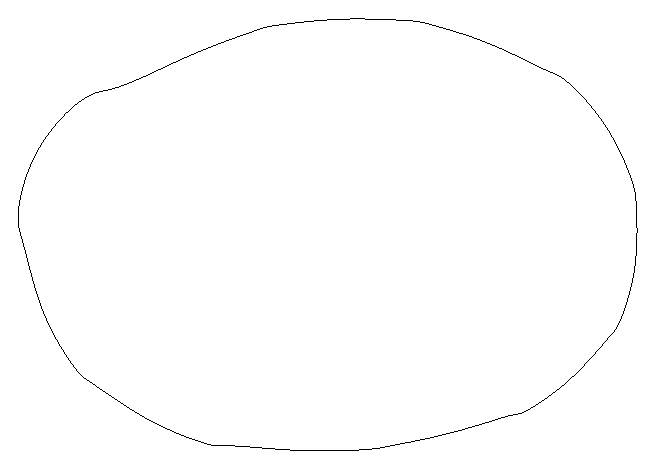
\includegraphics[width=\textwidth]{Domain}\\
  \end{minipage}%
  \begin{minipage}[b]{.33\linewidth}
  \centering
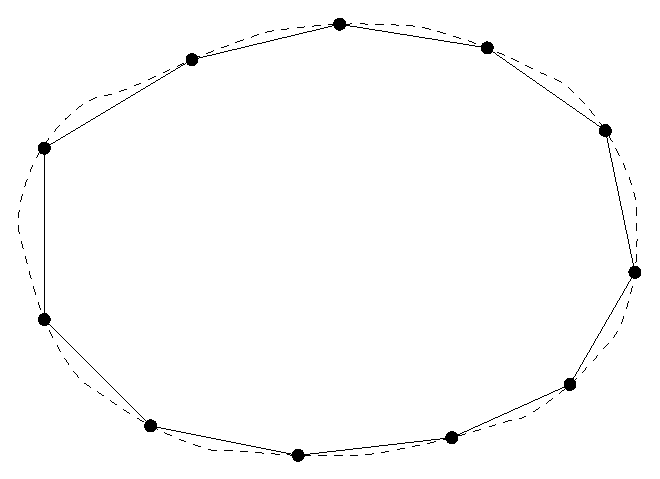
\includegraphics[width=\textwidth]{DomainPolygon}\\
  \end{minipage}%
    \begin{minipage}[b]{.33\linewidth}
  \centering
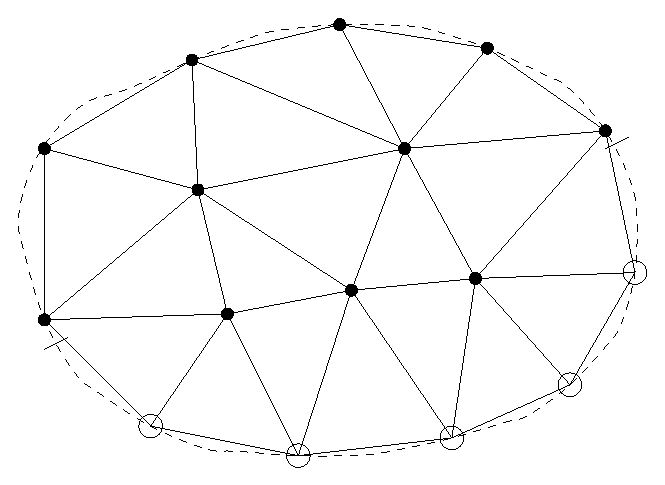
\includegraphics[width=\textwidth]{DomainBoundaryMesh}\\
  \end{minipage}
\end{figure} 


For any polygonal domain $\Omega$, $\Omega = \cup_{j} T_j$. The set of all elements are denoted by $\mathcal{T}_h$.

\end{frame}





      

%-=-=-=-=-=-=-=-=-=-=-=-=-=-=-=-=-=-=-=-=-=-=-=-=
%	FRAME:
%-=-=-=-=-=-=-=-=-=-=-=-=-=-=-=-=-=-=-=-=-=-=-=-=
\begin{frame}{Conforming and non conforming triangles}



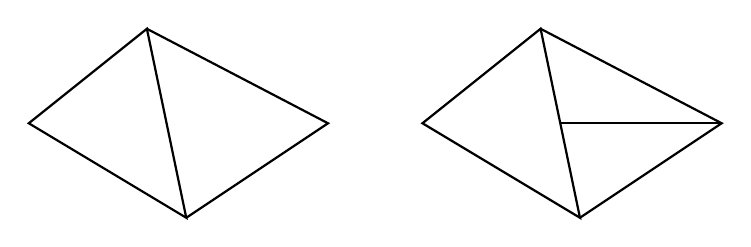
\begin{tikzpicture}




\draw[thick] (0, 0) -- (2, -1.2) -- (1.5, 1.2)--cycle;
\draw[thick] (2, -1.2) -- (3.8, 0) -- (1.5, 1.2);



\draw[thick] (5, 0) -- (7, -1.2) -- (6.5, 1.2)--cycle;
\draw[thick] (7, -1.2) -- (8.8, 0) -- (6.5, 1.2);
\draw [thick] (6.75, 0) -- (8.8, 0);
    \end{tikzpicture}
 
 
 
 \vspace{1em}
 
 Conforming triangulation $\mathcal{T}_h$:  $T_i\cap T_j \neq \emptyset \Rightarrow$ the intersection is either a \alert{vertex} of $T_i$ and $T_j$ or 
 the \alert{whole edge} of $T_i$ and $T_j$. 
 
\end{frame}







%-=-=-=-=-=-=-=-=-=-=-=-=-=-=-=-=-=-=-=-=-=-=-=-=
%	FRAME:
%-=-=-=-=-=-=-=-=-=-=-=-=-=-=-=-=-=-=-=-=-=-=-=-=
\begin{frame}{Linear finite element}

\begin{equation*}
	\boldsymbol{X}_{h}=\{\underbrace{v \in \boldsymbol{X}}_{\substack{ v \in C^{0}(\Omega)}}|v|_{\boldsymbol{T}} \in \mathbb{P}_{1}\left(\boldsymbol{T}\right), \forall \boldsymbol{T} \in \mathcal{T}_{h}\}
\end{equation*}


\begin{center}
	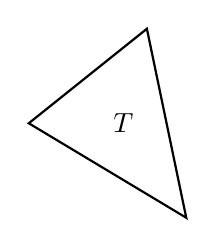
\begin{tikzpicture}
\draw[thick] (0, 0) -- (2, -1.2) -- (1.5, 1.2)--cycle;

\node at (1.2, 0) {$T$};

    \end{tikzpicture}
\end{center}
\begin{equation*}
	\mathbb{P}_{1}\left(T\right):\left.v\right|_{T_{h}}=c_{1}+\underbrace{c_{2}}_{v_{x}} x+\underbrace{c_{3}}_{v_{y}} y, \quad c_1, c_{2}, c_{3} \in \mathbb{R}
\end{equation*}


Need 3 basis functions per element. Need 3 DOF per element. 
 
\end{frame}






%-=-=-=-=-=-=-=-=-=-=-=-=-=-=-=-=-=-=-=-=-=-=-=-=
%	FRAME:
%-=-=-=-=-=-=-=-=-=-=-=-=-=-=-=-=-=-=-=-=-=-=-=-=
\begin{frame}{Mapping from canonical triangle to arbitrary element}

	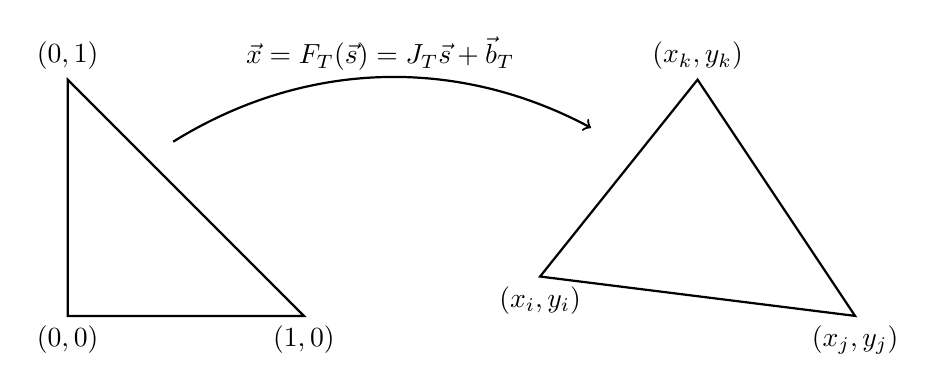
\begin{tikzpicture}
\draw[thick] (0, 0) -- (3, 0) -- (0, 3)--cycle;
\node at (0, 0) [below] {$(0, 0)$};
\node at (3, 0) [below] {$(1, 0)$};
\node at (0, 3) [above] {$(0, 1)$};


\draw[thick] (6, 0.5) -- (10, 0) -- (8, 3)--cycle;
\node at (6, 0.5) [below] {$(x_i, y_i)$};
\node at (10, 0) [below] {$(x_j, y_j)$};
\node at (8, 3) [above] {$(x_k, y_k)$};

\draw [->,shorten <=4mm,shorten >=4mm, thick] (1,2) to[bend left] node[above]{$\vec{x} = F_T(\vec{s}) = J_T\vec{s} + \vec{b}_T$} (7, 2.2);

    \end{tikzpicture}
 
\end{frame}









%-=-=-=-=-=-=-=-=-=-=-=-=-=-=-=-=-=-=-=-=-=-=-=-=
%	FRAME:
%-=-=-=-=-=-=-=-=-=-=-=-=-=-=-=-=-=-=-=-=-=-=-=-=
\begin{frame}{Construction of affine mapping}
 
 Mapping condition: 
 \begin{itemize}
 	\item  $F_T((0,0)) = (x_i, y_i)$,
 	\item  $F_T((1,0)) = (x_j, y_j)$,
 	\item  $F_T((0,1)) = (x_k, y_k)$.
 \end{itemize}



\begin{equation*}
\begin{bmatrix}
x\\
y
\end{bmatrix}
=
\begin{bmatrix}
x_j-x_i & x_k-x_i\\
y_j-y_i & y_k-y_i
\end{bmatrix}
\begin{bmatrix}
\xi\\
\eta
\end{bmatrix}
+
\begin{bmatrix}
x_i\\
y_i
\end{bmatrix}
\end{equation*}


\begin{equation*}
\Rightarrow \vec{x}=F_T(\vec{s}) ={J}_T\vec{s} +  \vec{b}_T.
\end{equation*}

 
\end{frame}




%-=-=-=-=-=-=-=-=-=-=-=-=-=-=-=-=-=-=-=-=-=-=-=-=
%	FRAME:
%-=-=-=-=-=-=-=-=-=-=-=-=-=-=-=-=-=-=-=-=-=-=-=-=
\begin{frame}{Nodal basis }

Nodal basis at reference element \mbox{$N_j(v_i)=\delta_{ij}$}(where $v_i$ are three vertices of reference element):
\begin{align*}
N_1(\xi,\eta)=&1-\xi-\eta,  \quad\quad\quad\quad
\nabla_{\vec{s}}N_1 = \begin{pmatrix}
	-1 \\ -1
\end{pmatrix}, \\
N_2(\xi,\eta)=&\xi,  \quad\quad\quad\quad\quad\quad\quad\quad
\nabla_{\vec{s}}N_2 = \begin{pmatrix}
	1 \\ 0
\end{pmatrix},\\
N_3(\xi,\eta)=&\eta, \quad\quad\quad\quad\quad\quad\quad\quad
\nabla_{\vec{s}}N_3 = \begin{pmatrix}
	0 \\ 1
\end{pmatrix}.
\end{align*}

	
	
Nodal basis at general element: $\phi_j(x,y) = N_j(F_T^{-1}(x,y))$.
	
	
\end{frame}




%-=-=-=-=-=-=-=-=-=-=-=-=-=-=-=-=-=-=-=-=-=-=-=-=
%	FRAME:
%-=-=-=-=-=-=-=-=-=-=-=-=-=-=-=-=-=-=-=-=-=-=-=-=
\begin{frame}{Evaluation of basis function at general element}
Observation: $\phi_j(x,y) = N_j(F_T^{-1}(x,y)) \Leftrightarrow \phi_j(F_T(\xi, \eta)) = N_j(\xi,\eta)$.
\vspace{1em}


Chain rule: $$\frac{\partial N_j}{\partial \xi} = \frac{\partial }{\partial \xi}\phi_j(F_T(\xi, \eta)) = \frac{\partial \phi_j}{\partial x}\frac{\partial x}{\partial \xi} + \frac{\partial \phi_j}{\partial y}\frac{\partial y}{\partial \xi}=  \frac{\partial \phi_j}{\partial x}J_{11} + \frac{\partial \phi_j}{\partial y}J_{21}$$

Similarly, 
	$$\frac{\partial N_j}{\partial \eta} = \frac{\partial }{\partial \eta}\phi_j(F_T(\xi, \eta)) =   \frac{\partial \phi_j}{\partial x}J_{12} + \frac{\partial \phi_j}{\partial y}J_{22}$$
	
Combining those, implies
\begin{equation*}
	\begin{bmatrix}
		\frac{\partial N_j}{\partial \xi} \\ 
		\frac{\partial N_j}{\partial \eta}
	\end{bmatrix}
	= \begin{bmatrix}
		J_{11}\frac{\partial \phi_j}{\partial x} + J_{21}\frac{\partial \phi_j}{\partial y}\\
		J_{12}\frac{\partial \phi_j}{\partial x} + J_{22}\frac{\partial \phi_j}{\partial y}
	\end{bmatrix}
	 = \begin{bmatrix}
	 	J_{11} & J_{21}\\ J_{12} & J_{22}
	 \end{bmatrix}
	 \begin{bmatrix}
	 	\frac{\partial \phi_j}{\partial x} \\ \frac{\partial \phi_j}{\partial y}
	 \end{bmatrix}
\end{equation*}
	In other words, $\nabla_{\vec{s}}N_j = J^{T}_{T} \nabla \phi_j
\Rightarrow 	\nabla \phi_j = J^{-T}_{T}\nabla_{\vec{s}}N_j $.

	
	
\end{frame}



%-=-=-=-=-=-=-=-=-=-=-=-=-=-=-=-=-=-=-=-=-=-=-=-=
%	FRAME:
%-=-=-=-=-=-=-=-=-=-=-=-=-=-=-=-=-=-=-=-=-=-=-=-=
\begin{frame}{Computation of element load vector}
Element load vector:
\begin{equation*}
f_{T}=
\begin{bmatrix}
\int_{T} f \phi_i \, dA\\
\int_{T} f \phi_{j} \, dA\\
\int_{T} f \phi_{k} \, dA
\end{bmatrix},
\end{equation*}


Calculate the entries as
\begin{align*}
\int_{T} f \phi_i \, dA = &\int_{T}f(\vec{x})\phi_j(\vec{x})\, dxdy\\
=&\int_{T_R} f(\vec{x}(\vec{s}))N_j(\vec{s})|\mbox{det}(J_T)|\, d\xi d \eta.
\end{align*}	
	
\end{frame}



%-=-=-=-=-=-=-=-=-=-=-=-=-=-=-=-=-=-=-=-=-=-=-=-=
%	FRAME:
%-=-=-=-=-=-=-=-=-=-=-=-=-=-=-=-=-=-=-=-=-=-=-=-=
\begin{frame}{Computation of element stiffness matrix}
Element stiffness matrix, 
\begin{equation*}
K_{T}=
\begin{bmatrix}
\int_{T} D\nabla\phi_i\cdot\nabla\phi_i \, dA&
\int_{T} D\nabla\phi_i\cdot\nabla\phi_j \, dA&
\int_{T} D\nabla\phi_i\cdot\nabla\phi_k \, dA&\\
\int_{T} D\nabla\phi_j\cdot\nabla\phi_i \, dA&
\int_{T} D\nabla\phi_j\cdot\nabla\phi_j \, dA&
\int_{T} D\nabla\phi_j\cdot\nabla\phi_k \, dA&\\
\int_{T} D\nabla\phi_k\cdot\nabla\phi_i \, dA&
\int_{T} D\nabla\phi_k\cdot\nabla\phi_j \, dA&
\int_{T} D\nabla\phi_k\cdot\nabla\phi_k \, dA&\\
\end{bmatrix},
\end{equation*}


Calculate the entries as
\begin{align*}
\int_{T}  D\nabla\phi_i\cdot\nabla & \phi_j \, dA 
= \int_{T} D(\vec{x})\nabla\phi_i(\vec{x})\cdot\nabla\phi_j(\vec{x})\, dxdy\\
= &\int_{T_R} D(\vec{x}(\vec{s}))\left(J_T^{-T}\nabla_{\vec{s}}N_i(\vec{s})\right)\cdot\left(J_T^{-T}\nabla_{\vec{s}} N_j(\vec{s})\right)|\operatorname{det}(J_T)|\, d\xi d\eta.
\end{align*}
	
	
\end{frame}




%-=-=-=-=-=-=-=-=-=-=-=-=-=-=-=-=-=-=-=-=-=-=-=-=
%	FRAME:
%-=-=-=-=-=-=-=-=-=-=-=-=-=-=-=-=-=-=-=-=-=-=-=-=
\begin{frame}{Quadrature  rules on triangle }
Some quadrature rules on reference triangles $T_R$:
\begin{itemize}
	\item $\int_{T_R}g(\xi,\eta)d\xi d\eta \approx \frac{1}{2}g(1/3,1/3)$,
	
	\item $\int_{T_R}g(\xi,\eta)d\xi d\eta \approx
	 \frac{1}{6}\left[g(1/2,0) + g(1/2,1/2) + g(0, 1/2)\right]$,

\end{itemize}
	
	
\end{frame}

%-=-=-=-=-=-=-=-=-=-=-=-=-=-=-=-=-=-=-=-=-=-=-=-=
%	FRAME:
%-=-=-=-=-=-=-=-=-=-=-=-=-=-=-=-=-=-=-=-=-=-=-=-=
\begin{frame}{Data structure for implementing linear 2D FEM}





\begin{columns}
\begin{column}{.4\textwidth}
\begin{center}
	    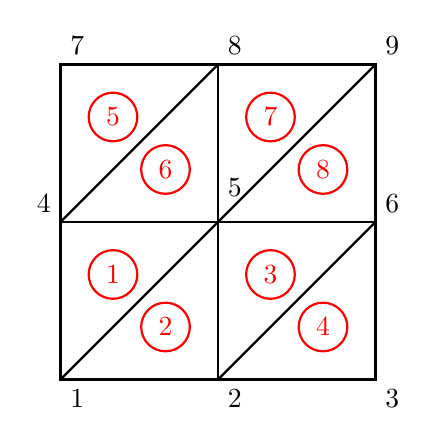
\begin{tikzpicture}


 \draw [black, thick] (0,0) rectangle (4,4);

    
\draw [thick] (2,0) -- (2, 4);  
    
\draw [thick] (0,2) -- (4, 2);
   
\draw [thick] (0,0) -- (4, 4);
\draw [thick] (2,0) -- (4, 2);
\draw [thick] (0,2) -- (2, 4);



   \node[draw,circle,thick,color=red] (CircleNode) at (4/3,2/3)  {$2$};
    \node[draw,circle,thick,color=red] (CircleNode) at (2/3,4/3)  {$1$};
   \node[draw,circle,thick,color=red] (CircleNode) at (10/3,2/3)  {$4$};
   \node[draw,circle,thick,color=red] (CircleNode) at (8/3,4/3)  {$3$};

  \node[draw,circle,thick,color=red] (CircleNode) at (4/3,8/3)  {$6$};
    \node[draw,circle,thick,color=red] (CircleNode) at (2/3,10/3)  {$5$};
   \node[draw,circle,thick,color=red] (CircleNode) at (10/3,8/3)  {$8$};
   \node[draw,circle,thick,color=red] (CircleNode) at (8/3,10/3)  {$7$};

 \node at (0, 0) [below right] {$1$};
\node at (2, 0) [below right]  {$2$};
\node at (4, 0) [below right]  {$3$};
 \node at (0, 2) [above left] {$4$};
\node at (2, 2.2) [above right]  {$5$};
\node at (4, 2) [above right]  {$6$};
 \node at (0, 4) [above right] {$7$};
\node at (2, 4) [above right]  {$8$};
\node at (4, 4) [above right]  {$9$};


\end{tikzpicture}
\end{center}



\end{column}

\begin{column}{.6\textwidth}



\begin{equation*}
\text{node} =
\begin{bmatrix}
	0 & 0\\
	\frac{1}{2} & 0\\
	1 & 0 \\
0 & \frac{1}{2}\\
	\frac{1}{2} & \frac{1}{2}\\
	1 & \frac{1}{2} \\
	0 & 1\\
	\frac{1}{2} & 1\\
	1 & 1 \\
	\end{bmatrix}
	\quad \quad
	\text{elem} = \begin{bmatrix}
	1 & 5 & 4 \\
	1 & 2 & 5\\
	2 & 6 & 5\\
	2 & 3 & 6\\
	4 & 8 & 7\\
	4 & 5 & 8\\
	5 & 9 & 8\\
	5 & 6 & 9
\end{bmatrix}
\end{equation*}


 



\end{column}

\end{columns}


$node$ and $elem$ can be also  generated using mesh generator like \textbf{distmesh}
 and \textbf{triangle}.


\end{frame}





%-=-=-=-=-=-=-=-=-=-=-=-=-=-=-=-=-=-=-=-=-=-=-=-=
%	FRAME:
%-=-=-=-=-=-=-=-=-=-=-=-=-=-=-=-=-=-=-=-=-=-=-=-=
\begin{frame}{Pseudo code}


N = size(node,1);  NT = size(elem,1)

A = sparse(N, N); b = zeros(N,1);


for j = 1:NT



$\quad\quad P1 = node(elem(j,1), :);$



$\quad\quad P2 = node(elem(j,2), :);$



$\quad\quad P3 = node(elem(j,3), :);$


$\quad\quad K_{E_j} = elem\_stiff(P1,P2,P3,D); $ \% compute local stiffness matrix



$\quad\quad F_{E_j} = elem\_load(P1,P2,P3, f); $ \% compute local load vector



$\quad\quad A(elem(j,:), elem(j,:)) = A(elem(j,:), elem(j,:)) + K_{E_j}; $ 



$\quad\quad b(elem(j,:), 1) = b(elem(j,:), 1) + F_{E_j}; $ 



end





You should write functions to compute element matrices/vectors which can be done by mapping into master element. 

\end{frame}




%-=-=-=-=-=-=-=-=-=-=-=-=-=-=-=-=-=-=-=-=-=-=-=-=
%	FRAME:
%-=-=-=-=-=-=-=-=-=-=-=-=-=-=-=-=-=-=-=-=-=-=-=-=
\begin{frame}{Impose Dirichlet boundary condition}

Need identify boundary nodes. 


\vspace{0.5em}

On rectangle domain $[a, b]\times [c, d]$:

$isLeftBnd = abs(node(:,1)-a)<eps$



$isRightBnd = abs(node(:,1)-b)<eps$



$isButtomBnd = abs(node(:,2)-c)<eps$


$isTopBnd = abs(node(:,2)-d)<eps$



\end{frame}



%-=-=-=-=-=-=-=-=-=-=-=-=-=-=-=-=-=-=-=-=-=-=-=-=
%	FRAME:
%-=-=-=-=-=-=-=-=-=-=-=-=-=-=-=-=-=-=-=-=-=-=-=-=
\begin{frame}{Impose Dirichlet boundary condition (continue)}



$isBndNode = false(N,1);$



$isBndNode(isLeftBnd) = true;$



$isBndNode(isRightBnd) = true;$


$isBndNode(isButtomBnd) = true;$


$isBndNode(isTopBnd) = true;$


$bndNode = find(isBndNode);$


$freeNode = find(\sim isBndNode);$


$u = zeros(N,1);$

$u(bndNode) = g_D(node(bndNode,:));$


$b = b - A*u;$


$ u(freeNode) = A(freeNode, freeNode) \backslash b(freeNode);$



Other useful \textbf{MATLAB} command: $trimesh$,  $triplot$,  and $trisurf$.

\end{frame}



%-=-=-=-=-=-=-=-=-=-=-=-=-=-=-=-=-=-=-=-=-=-=-=-=
%	FRAME:
%-=-=-=-=-=-=-=-=-=-=-=-=-=-=-=-=-=-=-=-=-=-=-=-=
\begin{frame}{Theoretical analysis: Energy norm}

From the bilinear form we define an energy norm

$\|v\|^{2}_{E} \equiv a(v, v)$. 
Then
$$
\|u-u_h\|_{E}=\inf_{w_{h} \in X_{h}} \|u-w_{h}\|_{E}
$$

$u$ is the solution to the PDE and $u_{h}$ is the projection of $u$ on $\boldsymbol{X}_{h}$ with respect to the bilinear form.

$\inf$ is the infimum, i.e., the maximal lower bound. 

\end{frame}



%-=-=-=-=-=-=-=-=-=-=-=-=-=-=-=-=-=-=-=-=-=-=-=-=
%	FRAME:
%-=-=-=-=-=-=-=-=-=-=-=-=-=-=-=-=-=-=-=-=-=-=-=-=
\begin{frame}{Theoretical analysis: $H1$ norm}


Recall $\|v\|_{H^{1}(\Omega)}^{2}=\int_{\Omega}|\nabla v|^{2}+v^{2} d A$
Then
$$
\|u-u_h\|_{H^{1}(\Omega)} \leq\left(1+\frac{\beta}{\alpha}\right) \inf _{w_{h} \in X_{h}}\left\|u-w_{h}\right\|_{H^{1}(\Omega)}
$$
$\alpha$: coercivity constant $(>0)$;
$\beta$: continuity constant $(=1)$.


\end{frame}



%-=-=-=-=-=-=-=-=-=-=-=-=-=-=-=-=-=-=-=-=-=-=-=-=
%	FRAME:
%-=-=-=-=-=-=-=-=-=-=-=-=-=-=-=-=-=-=-=-=-=-=-=-=
\begin{frame}{Theoretical analysis: $H1$ and $L2$ norm}


For $f \in L^{2}(\Omega)$ and $\Omega$ convex,
$$
\begin{aligned}
&\|u-u_h\|_{E} \leq C h\|u\|_{H^{2}(\Omega)} \\
&\|u-u_h\|_{H^{1}(\Omega)} \leq C h\|u\|_{H^{2}(\Omega)} \\
\text { and } \quad &\|u-u_h\|_{L^{2}(\Omega)} \leq C h^{2}\|u\|_{H^{2}(\Omega)}
\end{aligned}
$$


\end{frame}





%-=-=-=-=-=-=-=-=-=-=-=-=-=-=-=-=-=-=-=-=-=-=-=-=
%	FRAME:
%-=-=-=-=-=-=-=-=-=-=-=-=-=-=-=-=-=-=-=-=-=-=-=-=
\begin{frame}{Quadratic Lagrange element}


\begin{columns}
\begin{column}{.4\textwidth}
\begin{center}
	    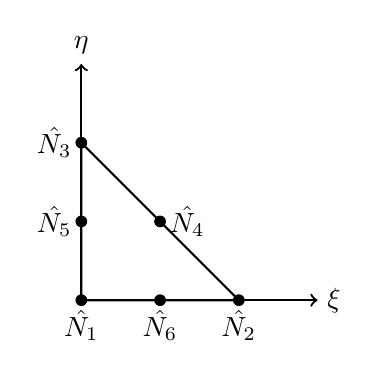
\begin{tikzpicture}


 

    
\draw [thick] (0,0) -- (2,0) -- (0,2) -- cycle;  
    
\draw [<->, thick] (3,0) -- (0,0) -- (0,3);

\node at (3, 0) [right] {$\xi$};

\node at (0, 3) [above] {$\eta$};





\node at (0, 0) [circle,fill,inner sep=1.5pt] {};
\node at (0, 2) [circle,fill,inner sep=1.5pt] {};
\node at (0, 1) [circle,fill,inner sep=1.5pt] {};
\node at (1, 1) [circle,fill,inner sep=1.5pt] {};
\node at (1, 0) [circle,fill,inner sep=1.5pt] {};
\node at (2, 0) [circle,fill,inner sep=1.5pt] {};





  \node at (0, 0) [below] {$\hat{N_1}$};
  
  
    \node at (2, 0) [below] {$\hat{N_2}$};


    \node at (0, 2) [left] {$\hat{N_3}$};



 \node at (1, 1) [right] {$\hat{N_4}$};
  
  
    \node at (0, 1) [left] {$\hat{N_5}$};


    \node at (1, 0) [below] {$\hat{N_6}$};


\end{tikzpicture}
\end{center}



\end{column}

\begin{column}{.6\textwidth}

$N_j$ shape function for linear element.

\vspace{0.5em}

$\hat{N_1} = N_1(1-2N_1)\quad \hat{N}_4 = 4N_2N_3 $
\vspace{0.5em}



$\hat{N_2} = N_2(1-2N_2)\quad \hat{N}_5 = 4N_1N_3 $

\vspace{0.5em}

$\hat{N_3} = N_3(1-2N_3)\quad \hat{N}_6 = 4N_1N_2 $

\end{column}
\end{columns}

\end{frame}



%-=-=-=-=-=-=-=-=-=-=-=-=-=-=-=-=-=-=-=-=-=-=-=-=
%	FRAME:
%-=-=-=-=-=-=-=-=-=-=-=-=-=-=-=-=-=-=-=-=-=-=-=-=
\begin{frame}{Bilinear element Q1}



\begin{columns}
\begin{column}{.4\textwidth}
\begin{center}
	    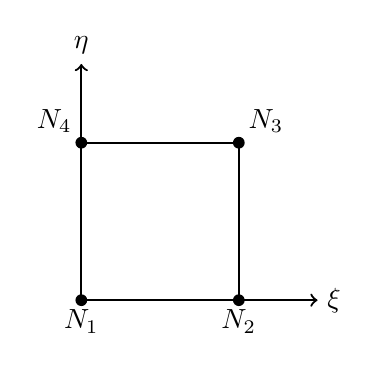
\begin{tikzpicture}


 

    
\draw [thick] (0,0) -- (2,0) -- (2,2) -- (0, 2)--  cycle;  
    
\draw [<->, thick] (3,0) -- (0,0) -- (0,3);

\node at (3, 0) [right] {$\xi$};

\node at (0, 3) [above] {$\eta$};





\node at (0, 0) [circle,fill,inner sep=1.5pt] {};
\node at (0, 2) [circle,fill,inner sep=1.5pt] {};
\node at (2, 2) [circle,fill,inner sep=1.5pt] {};
\node at (2, 0) [circle,fill,inner sep=1.5pt] {};





  \node at (0, 0) [below] {${N_1}$};
  
  
    \node at (2, 0) [below] {${N_2}$};


    \node at (2, 2) [above right] {${N_3}$};



 \node at (0, 2) [above left] {${N_4}$};
  



\end{tikzpicture}
\end{center}



\end{column}

\begin{column}{.6\textwidth}


\vspace{0.5em}

$N_1 = (1-\xi)(1-\eta) $
\vspace{0.5em}



$N_2 = (1-\xi)\eta $

\vspace{0.5em}

$N_3 = \xi(1-\eta) $



\vspace{0.5em}

$N_3 = \xi\eta $

\end{column}
\end{columns}


\end{frame}




%-=-=-=-=-=-=-=-=-=-=-=-=-=-=-=-=-=-=-=-=-=-=-=-=
%	FRAME:
%-=-=-=-=-=-=-=-=-=-=-=-=-=-=-=-=-=-=-=-=-=-=-=-=
\begin{frame}[standout]
  End of week 6!
\end{frame}

\appendix



\end{document}
